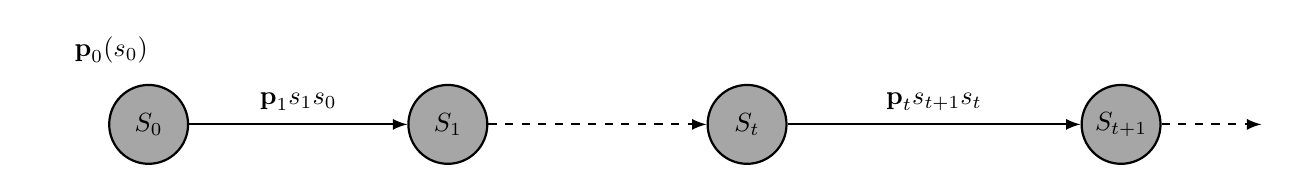
\begin{tikzpicture}[transform shape,scale=0.95]
% vertex shape and color
\tikzstyle{vertex}=[circle,fill=black!35,minimum size=30pt,inner sep=0pt, draw=black,thick]

% nodes
\node (left) at (-1.5,0) {};
\foreach \name/\x in {S_0/0,S_1/4,S_t/8, S_{t+1}/13}
\node[vertex] (G-\name) at (\x,0) {$\name$};
\node (G-end) at (15,0) {};

% arrows
\foreach \from/\to in {S_0/S_1,S_t/S_{t+1}}
\draw[->,>=latex,thick] (G-\from) -- (G-\to);
\foreach \from/\to in {S_1/S_t,S_{t+1}/end}
\draw[->,>=latex,dashed,thick] (G-\from) -- (G-\to);

% transition probabilities
\node (proba0) at (-0.5,1) {$\textbf{p}_0(s_0)$};
\node (proba1) at (2,0.3) {$\textbf{p}_1 \paren{ s_{1} \sachant s_{0}}$};
\node (probat) at (10.5,0.3) {$\textbf{p}_t \paren{ s_{t+1} \sachant s_{t}}$};
\end{tikzpicture}
